% Paper 1 (ICIMPACT 2027) — draf. Angka berasal dari angka.tex (dibuat angka.py dari cache).
% Template: IEEEtran conference (panitia: "IEEE Conference Template", maks. 6 halaman termasuk referensi, review blind).
% \blindtrue = versi anonim untuk submisi EDAS; \blindfalse = versi bernama untuk camera-ready.
\newif\ifblind
\blindtrue
\documentclass[conference,a4paper]{IEEEtran}
\IEEEoverridecommandlockouts
\usepackage[utf8]{inputenc}
\usepackage[T1]{fontenc}
\usepackage{amsmath,amssymb}
\usepackage{graphicx}
\usepackage{booktabs}
\usepackage{array}
\usepackage{tabularx}
\usepackage{xcolor}
\usepackage{cite}
\usepackage[hidelinks]{hyperref}
% Dibuat otomatis oleh angka.py dari cache. Jangan diedit manual.
\newcommand{\mfA}{\ensuremath{0.826}}
\newcommand{\sdA}{\ensuremath{0.084}}
\newcommand{\mfB}{\ensuremath{0.828}}
\newcommand{\sdB}{\ensuremath{0.086}}
\newcommand{\mfD}{\ensuremath{0.803}}
\newcommand{\sdD}{\ensuremath{0.130}}
\newcommand{\mfE}{\ensuremath{0.873}}
\newcommand{\ciE}{[0.72, 0.92]}
\newcommand{\aflPE}{\ensuremath{0.745}}
\newcommand{\aflRE}{\ensuremath{0.815}}
\newcommand{\mfF}{\ensuremath{0.786}}
\newcommand{\ciF}{[0.66, 0.85]}
\newcommand{\aflPF}{\ensuremath{0.371}}
\newcommand{\aflRF}{\ensuremath{0.812}}
\newcommand{\dF}{$-$0.087}
\newcommand{\dciF}{[$-$0.115, $-$0.052]}
\newcommand{\dpF}{0.000}
\newcommand{\mfG}{\ensuremath{0.759}}
\newcommand{\ciG}{[0.66, 0.83]}
\newcommand{\aflPG}{\ensuremath{0.264}}
\newcommand{\aflRG}{\ensuremath{0.812}}
\newcommand{\dG}{$-$0.026}
\newcommand{\dciG}{[$-$0.038, 0.002]}
\newcommand{\dpG}{0.033}
\newcommand{\mfH}{\ensuremath{0.759}}
\newcommand{\ciH}{[0.66, 0.83]}
\newcommand{\aflPH}{\ensuremath{0.263}}
\newcommand{\aflRH}{\ensuremath{0.812}}
\newcommand{\dH}{0.000}
\newcommand{\dciH}{[$-$0.001, 0.001]}
\newcommand{\dpH}{0.388}
\newcommand{\mfI}{\ensuremath{0.744}}
\newcommand{\ciI}{[0.64, 0.81]}
\newcommand{\aflPI}{\ensuremath{0.275}}
\newcommand{\aflRI}{\ensuremath{0.728}}
\newcommand{\dI}{$-$0.016}
\newcommand{\dciI}{[$-$0.028, $-$0.006]}
\newcommand{\dpI}{0.000}
\newcommand{\mfJ}{\ensuremath{0.418}}
\newcommand{\ciJ}{[0.36, 0.48]}
\newcommand{\aflPJ}{\ensuremath{0.027}}
\newcommand{\aflRJ}{\ensuremath{0.410}}
\newcommand{\dJ}{$-$0.325}
\newcommand{\dciJ}{[$-$0.427, $-$0.200]}
\newcommand{\dpJ}{0.000}
\newcommand{\dWindows}{$-$0.114}
\newcommand{\dPartition}{$-$0.025}
\newcommand{\dPooled}{$+$0.070}
\newcommand{\adF}{\ensuremath{0.087}}
\newcommand{\adG}{\ensuremath{0.026}}
\newcommand{\adI}{\ensuremath{0.016}}
\newcommand{\adJ}{\ensuremath{0.325}}
\newcommand{\adWindows}{\ensuremath{0.114}}
\newcommand{\adPartition}{\ensuremath{0.025}}
\newcommand{\adPooled}{\ensuremath{0.070}}
\newcommand{\maxRecE}{\ensuremath{0.04}}
\newcommand{\maxRecF}{\ensuremath{0.00}}
\newcommand{\biasShare}{80}
\newcommand{\nSeeds}{100}
\newcommand{\nPartitions}{1}
\newcommand{\sklearnVersion}{1.9.1}
\newcommand{\nAflLab}{4,925}
\newcommand{\nAflThin}{991}
\newcommand{\nAflDet}{1,152}
\newcommand{\nNormLab}{97,187}
\newcommand{\nAfLab}{32,810}
\newcommand{\nNormDet}{99,000}
\newcommand{\nAfDet}{65,826}
\newcommand{\refMF}{\ensuremath{0.832}}
\newcommand{\refCI}{[0.67, 0.92]}
\newcommand{\refAflF}{\ensuremath{0.647}}
\newcommand{\refAflCI}{[0.17, 0.89]}
\newcommand{\mfPone}{\ensuremath{0.779}}
\newcommand{\ciPone}{[0.63, 0.82]}
\newcommand{\gridOld}{\ensuremath{0.816}}
\newcommand{\gridNew}{\ensuremath{0.832}}
\newcommand{\biasAflMed}{$-$4.5}
\newcommand{\biasAflRange}{$-$5.5 to $-$4.0}
\newcommand{\normalRone}{\ensuremath{0.85}}
\newcommand{\normalRtwo}{\ensuremath{0.92}}
\newcommand{\share}{58}
\newcommand{\nPatients}{23}
\newcommand{\recA}{\ensuremath{0.40}}
\newcommand{\recB}{\ensuremath{0.92}}
\newcommand{\recC}{\ensuremath{0.51}}
\newcommand{\recD}{\ensuremath{0.17}}
\newcommand{\recE}{\ensuremath{0.00}}
\newcommand{\recF}{\ensuremath{0.00}}
\newcommand{\recG}{\ensuremath{0.96}}
\newcommand{\nWorse}{6}
\newcommand{\nNs}{6}
\newcommand{\nConfig}{12}
\newcommand{\mfBigruSoft}{\ensuremath{0.821}}
\newcommand{\dBigruSoft}{$-$0.010}
\newcommand{\pBigruSoft}{0.34}
\newcommand{\mfBigruFull}{\ensuremath{0.830}}
\newcommand{\dBigruFull}{$-$0.002}
\newcommand{\pBigruFull}{0.47}
\newcommand{\mfTcnFull}{\ensuremath{0.830}}
\newcommand{\dTcnFull}{$-$0.002}
\newcommand{\pTcnFull}{0.38}
\newcommand{\mfTcnSoft}{\ensuremath{0.752}}
\newcommand{\dTcnSoft}{$-$0.080}
\newcommand{\pTcnSoft}{0.03}
\newcommand{\dFixOne}{$+$0.088}
\newcommand{\ciFixOne}{[0.018, 0.164]}
\newcommand{\pFixOne}{0.98}
\newcommand{\dFixTwo}{$+$0.053}
\newcommand{\ciFixTwo}{[0.014, 0.120]}
\newcommand{\pFixTwo}{1.00}
\newcommand{\dWoOne}{$+$0.139}
\newcommand{\ciWoOne}{[$-$0.011, 0.181]}
\newcommand{\pWoOne}{0.94}
\newcommand{\dWoTwo}{$+$0.096}
\newcommand{\ciWoTwo}{[0.017, 0.127]}
\newcommand{\pWoTwo}{1.00}
\newcommand{\dNestOne}{$+$0.088}
\newcommand{\ciNestOne}{[0.005, 0.149]}
\newcommand{\pNestOne}{0.978}
\newcommand{\dNestTwo}{$+$0.053}
\newcommand{\ciNestTwo}{[0.007, 0.112]}
\newcommand{\pNestTwo}{0.993}
\newcommand{\tabelDekomposisi}{
A & Reported in the original notebook: one partition, per-fold mean, P0 windows & \mfA{} $\pm$ \sdA & -- & -- & -- \\
B & Re-run, same partition and recipe & \mfB{} $\pm$ \sdB & $+$0.002 & -- & -- \\
C & 5$\times$5 patient-level folds, per-fold mean & \mfD{} $\pm$ \sdD & \dPartition & -- & -- \\
D & Pooled out-of-fold predictions, P0 windows & \mfE{} \ciE & \dPooled & \aflPE & \aflRE \\
E & AFL test windows thinned from 1-s to $\geq$5-s stride & \mfF{} \ciF & \dF{} \dciF & \aflPF & \aflRF \\
F & AF test windows weighted $\times$2 (emulates 5-s stride) & \mfG{} \ciG & \dG{} \dciG & \aflPG & \aflRG \\
G & P1 window extraction, annotation R-peaks (250\,Hz) & \mfH{} \ciH & \dH{} \dciH & \aflPH & \aflRH \\
H & P1 window extraction, 50\,Hz detector R-peaks & \mfI{} \ciI & \dI{} \dciI & \aflPI & \aflRI \\
I & Originally deployed peak-finding front-end, no quality gate & \mfJ{} \ciJ & \dJ{} \dciJ & \aflPJ & \aflRJ \\
}


\begin{document}
\bstctlcite{IEEEexample:BSTcontrol}

\title{Where Did the F1 Go? A Fixed-Model Decomposition of Performance Inflation in RR-Interval Atrial Fibrillation and
Flutter Classification}

\ifblind
\author{\IEEEauthorblockN{Anonymous Author(s)}
\IEEEauthorblockA{Affiliation withheld for blind review}}
\else
\author{\IEEEauthorblockN{[Author 1], [Author 2], [Author 3], [Supervisor]}
\IEEEauthorblockA{\textit{[School / Faculty]}, \textit{Telkom University}, Bandung, Indonesia\\
\{[email]\}@[domain]}}
\fi

\maketitle

\begin{abstract}
Performance figures for RR-interval atrial fibrillation (AF) and atrial flutter (AFL) classifiers on the MIT-BIH Atrial
Fibrillation Database (AFDB) are hard to compare because evaluation choices vary. We reproduced a reported macro-F1 of \mfA{}
on a single patient partition (\mfB{} after retraining). In a separate analysis, we held 25 trained fold models fixed and
varied metric aggregation, test-window construction, R-peak source and front-end. Aligning test-window strides lowered pooled
macro-F1 from \mfE{} to \mfG{} (95\% CI \ciG), and thinning 1-s-stride AFL windows halved AFL precision. Switching from annotated
beats to a 50\,Hz detector lowered macro-F1 by \adI. The original peak-finding front-end without quality gating lowered it by
a further \adJ{} to \mfJ. In paired $5\times5$ patient-level cross-validation, none of the tested configurations outperformed
the recalibrated reference (\refMF{}, 95\% CI \refCI). Its advantage over the original recipe met the bootstrap improvement
criterion with all patients ($P=\pFixOne$) and became indistinguishable after excluding the patient who contributed
\share\% of detector AFL windows ($P=\pWoOne$). We provide a checklist for reporting test-window construction, patient-level
uncertainty and front-end performance.
\end{abstract}

\begin{IEEEkeywords}
atrial fibrillation, atrial flutter, RR interval, evaluation methodology, data leakage, reproducibility, wearable ECG
\end{IEEEkeywords}

\section{Introduction}
Detecting atrial fibrillation (AF) and atrial flutter (AFL) from wearable single-lead ECG is attractive because the inter-beat
(RR) interval sequence can be extracted on low-power hardware sampling at only 50\,Hz. AFL is rarer than AF and its 2:1
conduction pattern is regular, so it is the hardest of the three classes for RR-only methods. The MIT-BIH Atrial Fibrillation
Database (AFDB)~\cite{moody1983afdb,goldberger2000physionet} is the de facto benchmark, yet it contains only 23 usable records
and AFL occurs in just seven of them. With so few patients, the reported performance depends heavily on how the evaluation is
set up.

Prior work has shown that splitting windows rather than patients inflates AF-detection results~\cite{dechazal2004,
butkuviene2021,domazetoski2022}. Less is known about (i) how much each evaluation choice contributes when the trained models
are held fixed, (ii) how large the inflation can be \emph{without} any patient leakage, and (iii) how fragile ``model X is
better'' conclusions are on AFDB.

This paper is a case study from developing a three-class (Normal, AF, AFL) classifier for a 50\,Hz single-lead device. An
early pipeline reported a macro-F1 of \mfA{}. We first reproduced that score, then evaluated how the original recipe behaved
under a common set of patient folds. We ask how evaluation choices affect scores with fixed models, whether alternative
configurations improve on the recalibrated reference, and how much the comparisons depend on a dominant patient and on
decision-bias selection. We contribute the following.
\begin{itemize}
\item a reproduction of the original single-partition result and a separate fixed-model analysis showing how test-window
construction and the original R-peak front-end affected AFDB scores;
\item a paired comparison of twelve configurations of nine RR-interval models against the reference, in which none was better
and full class weights improved the TCN result;
\item quantified examples of fragile conclusions (single-patient dependence, nested bootstrap) and of a silent
cross-validation pitfall in a widely used library;
\item an evaluation checklist that extends existing recommendations~\cite{butkuviene2021,collins2024tripodai}.
\end{itemize}

\section{Related Work}
The inter-patient paradigm for ECG classification was established for beat classification~\cite{dechazal2004,luz2016}. For AF,
Butkuvien\.{e} et al.~\cite{butkuviene2021} found that only 4 of 14 deep-learning detectors evaluated on AFDB separated training
and test patients, and that a detector's specificity fell markedly once patients were separated. Domazetoski et
al.~\cite{domazetoski2022} reported that AFL sensitivity dropped from 71\% to 5.4\% when a random split was replaced by a patient
split. Illarionov and Khudorozhkov~\cite{illarionov2018} showed that intra-patient AFDB splits saturate with little training data,
and Seo et al.~\cite{seo2021} reported large accuracy losses across databases. Kapoor and Narayanan~\cite{kapoor2023} catalogue
leakage types, including sampling bias in the test distribution; overlapping windows inflate results in activity recognition and
EEG~\cite{dehghani2019,brookshire2024}. Forman and Scholz~\cite{forman2010} showed that averaging F1 over folds is biased compared
with pooling counts. RR-based AF detection degrades with noise and R-peak errors~\cite{oster2015}, and 50\,Hz sampling is
borderline for interval timing~\cite{kwon2018,ellis2015}. Benchmarks of many ECG architectures often find differences within
error bars~\cite{strodthoff2021,clifford2017}. Post-hoc selection should be repeated inside resampling~\cite{tsamardinos2018,
cawley2010}, and patient-clustered data call for patient-level bootstrap~\cite{rutter2000}. RR-based three-class AF/AFL
classifiers exist~\cite{ivanovic2019,faust2021}, but none of these studies decomposes an inflated figure while holding the models
fixed.

\section{Methods}
\subsection{Data and pipelines}
We used the 23 AFDB records with ECG signals and their rhythm annotations, keeping 10-s windows that lie within a single
Normal, AF or AFL segment. Normal denotes the AFDB \texttt{(N} rhythm label. Each window is represented by up to 30 RR intervals
(in ms) and their first differences, with padding masks. For the annotation-based sets, we used manually corrected
\texttt{.qrsc} beats when available and automated \texttt{.qrs} beats otherwise. Record 07859 required \texttt{.qrsc}.
We built the following window sets from the same records.
\begin{itemize}
\item \textbf{P0 windows} use annotated R-peaks at 250\,Hz. Strides of 5\,s for Normal, 10\,s for AF and 1\,s for AFL
yielded \nNormLab/\nAfLab/\nAflLab{} windows, respectively.
\item \textbf{P1 windows} (revised pipeline): uniform 5-s stride and a quality gate (RR 300--2000\,ms, at most one outlier, at
least four intervals), with R-peaks either from the annotations or from a detector run on the signal resampled to 50\,Hz
(detector: \nNormDet/\nAfDet/\nAflDet{} windows; \share\% of AFL windows from record 04936);
\item \textbf{deployed front-end}: the original backend, which resampled the 50\,Hz signal to 250\,Hz and applied a peak finder
(threshold at the signal mean, minimum distance 0.4\,s) without filtering or quality gating.
\end{itemize}

\subsection{Models}
The original recipe (P0) is a MicroTransformer with 8{,}739 parameters ($d_\text{model}=32$, two heads) trained with
class-weighted cross-entropy, AdamW (learning rate $10^{-3}$, weight decay $10^{-4}$), batch size 256 and 30 epochs with cosine
decay, using argmax decisions. The model zoo contains LightGBM on 16 HRV features, a masked ResNet1D, a BiGRU with attention, TCN,
InceptionTime, MiniRocket with logistic regression, XGBoost and an RBF SVM (Nystr\"om approximation). Deep models used either
full (inverse-frequency) or soft (square-root) class weights. Three pipelines are compared on the same P1 detector test
windows: P0 is the original recipe with argmax decisions (step H in Table~\ref{tab:decomp}); P1 is the MicroTransformer trained on
P1 windows with the fixed biases of the revised pipeline (0, $+2$, $-3$ for Normal, AF, AFL), which had been selected on a grid
of $-3$ to $+3$; and the recalibrated reference P2 uses the same out-of-fold probabilities as P1 with cross-fitted biases on the
wider grid described below.

\subsection{Evaluation protocol}
Patients were assigned to five folds by stratified round-robin (AFL patients, AF-dominant patients, others), repeated five times
(seed 2026). Metrics were computed from pooled out-of-fold predictions within each repeat and averaged over repeats. 95\% CIs come
from 2{,}000 stratified patient-bootstrap resamples; paired comparisons use identical resamples, and $P$ is the fraction of
resamples with $\Delta>0$, a bootstrap probability rather than a $p$-value (verdict: better if $P\geq0.95$, worse if
$P\leq0.05$, otherwise not distinguishable). Decision biases are additive log-probability
offsets per class chosen on the other folds (cross-fit) from a grid of $-7$ to $+3$ that maximises macro-F1.

\subsection{Fixed-model decomposition}
Step A in Table~\ref{tab:decomp} is the reported single-partition result. For step B we retrained five models using the
original splitter settings and the P0 recipe. For steps C--I we trained 25 models on the P0 windows of the $5\times5$ design
and held them fixed, applying each model to the same held-out patients across test sets. Step E keeps AFL test windows at
least 5\,s apart within a record (\nAflLab{} $\rightarrow$ \nAflThin{} windows). Step F weights AF test windows by two to emulate
a 5-s stride. The repeated training reproduced the cached class decisions exactly on the three test sets previously evaluated.

\subsection{Robustness analyses}
We repeated paired comparisons with a nested bootstrap that re-selects the decision biases inside every resample, in the
spirit of BBC-CV~\cite{tsamardinos2018}. In a separate sensitivity analysis we excluded record 04936 from scoring and bias
selection using the existing fold models. We also report per-patient AFL recall.

\section{Results}
\subsection{Decomposing an inflated number}
\begin{table*}[t]
\centering
\caption{Fixed-model decomposition of the P0 macro-F1. Steps A--C: per-fold mean $\pm$ SD across folds; steps D--I: pooled
out-of-fold value with 95\% patient-bootstrap CI; $\Delta$ relative to the previous step (95\% CI for E--I). AFL P/R: AFL
precision/recall.}
\label{tab:decomp}
\footnotesize
\begin{tabularx}{\textwidth}{c X c c c c}
\toprule
Step & Evaluation condition & Macro-F1 & $\Delta$ & AFL P & AFL R \\
\midrule
\tabelDekomposisi
\bottomrule
\end{tabularx}
\end{table*}

\begin{figure}[t]
\centering
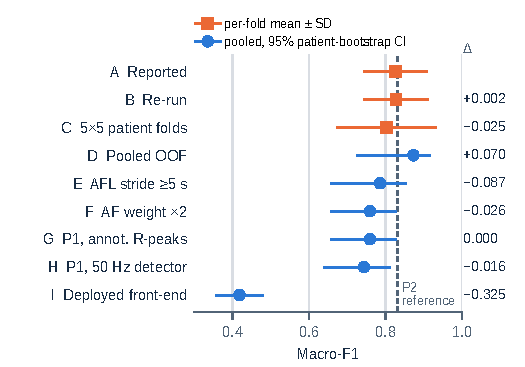
\includegraphics[width=\columnwidth]{gambar/dekomposisi.pdf}
\caption{Macro-F1 of P0 models under successive evaluation conditions (steps as in Table~\ref{tab:decomp}; C--I use the same
25 fold models). The dashed line is the recalibrated reference (P2).}
\label{fig:decomp}
\end{figure}

Table~\ref{tab:decomp} and Fig.~\ref{fig:decomp} trace the reported figure. Re-running the original recipe with the original
splitter settings gave a similar score (\mfB{} vs \mfA), with close agreement across folds. Moving to $5\times5$ patient-level
folds with newly trained models lowered the fold-averaged score by \adPartition{} and raised the across-fold SD to \sdD.
For the 25 models in this design, pooling out-of-fold predictions raised macro-F1 by \adPooled{} relative to averaging
per-fold scores. The two estimators weight the underlying counts differently~\cite{forman2010}.

Class-specific test strides inflated the score even with patients separated between training and test. Thinning the
1-s-stride AFL test windows (E) lowered macro-F1 by \adF{} (95\% CI for $\Delta$ \dciF), halving AFL precision
(\aflPE{} to \aflPF) while AFL recall changed little (\aflRE{} to \aflRF). Dense AFL windows give more weight to true positives,
while the non-AFL windows that contribute false positives are held fixed in this step. Emulating the 5-s AF stride (F) cost
another \adG. The resulting score closely matched the P1 extraction with annotation R-peaks (G, difference \dH), and both
sets contained \nAflThin{} AFL windows. Switching to the 50\,Hz detector pipeline (H) lowered macro-F1 by \adI{} and AFL
recall from \aflRH{} to \aflRI. Switching to the original front-end (I) produced the largest drop, \adJ, and lowered AFL
precision to \aflPJ.

A library default caused a further problem that produced no warning. With scikit-learn \sklearnVersion, \texttt{StratifiedGroupKFold(shuffle=True)} produced
\nPartitions{} patient partition for \nSeeds{} different seeds on both window sets, because shuffling only reorders groups whose
class-distribution spread is exactly tied~\cite{sklearn32478}. ``Repeated'' cross-validation with different seeds was therefore
not repeated. Versions before 1.8 instead shuffled class counts without their groups, yielding random, unstratified partitions.
Our round-robin assignment produced five distinct partitions in five repeats.

\subsection{Comparing model architectures and training recipes}
\begin{figure}[t]
\centering
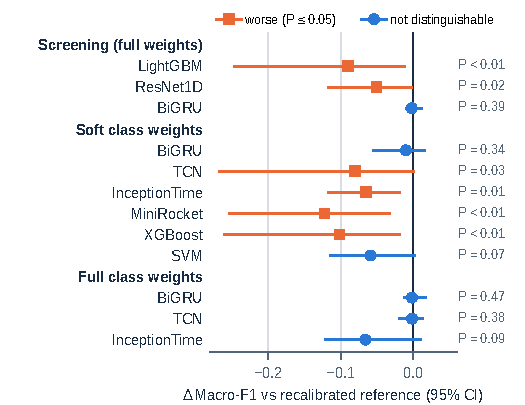
\includegraphics[width=\columnwidth]{gambar/forest.pdf}
\caption{Paired difference in macro-F1 between each configuration and the recalibrated reference (MicroTransformer with
cross-fitted biases), with 95\% patient-bootstrap CIs and $P(\Delta>0)$.}
\label{fig:forest}
\end{figure}

Fig.~\ref{fig:forest} compares \nConfig{} configurations of nine models (including two BiGRU implementations) with the reference
(\refMF, \refCI; AFL F1 \refAflF, \refAflCI). None was better; \nWorse{} were worse and \nNs{} were not distinguishable. With soft class weights, the BiGRU was
the best model (\mfBigruSoft, $\Delta$=\dBigruSoft, $P=\pBigruSoft$) and the TCN was worse ($\Delta$=\dTcnSoft, $P=\pTcnSoft$);
with full class weights both reached \mfBigruFull{} ($\Delta$=\dBigruFull{} and \dTcnFull). The change from soft to full weights
for the TCN was larger than the difference between the two architectures at full weights. Adding cross-fitted biases to the
original P0 models alone recovered \biasShare\% of the reference's improvement over P0.

The width of the bias grid mattered as well. The revised pipeline (P1) selected biases on a grid of $-3$ to $+3$; the optimal AFL
bias lies at \biasAflRange{} (median \biasAflMed), so the search hit the boundary and compensated by raising the AF bias, which
lowered Normal recall to \normalRone{} (reference: \normalRtwo). Widening the grid raised macro-F1 from \gridOld{} to \gridNew,
so an optimum at the grid boundary signals that the grid is too narrow.

\subsection{Fragile conclusions}
\begin{table}[t]
\centering
\caption{Paired macro-F1 differences of the reference (P2) against the original (P0) and revised (P1) pipelines.}
\label{tab:robust}
\footnotesize
\setlength{\tabcolsep}{3pt}
\begin{tabular}{l c c}
\toprule
Analysis & P2 $-$ P0 & P2 $-$ P1 \\
\midrule
Fixed biases, all patients & \dFixOne{} ($P$=\pFixOne) & \dFixTwo{} ($P$=\pFixTwo) \\
Nested bootstrap & \dNestOne{} ($P$=\pNestOne) & \dNestTwo{} ($P$=\pNestTwo) \\
Without record 04936 & \dWoOne{} ($P$=\pWoOne) & \dWoTwo{} ($P$=\pWoTwo) \\
\bottomrule
\end{tabular}
\end{table}

With all patients included, repeating bias selection within each bootstrap resample lowered support for P2 over P1
from $P=\pFixTwo$ to $P=\pNestTwo$. Both analyses met the improvement criterion. The P2 vs P0 result changed from better
with all patients ($P=\pFixOne$) to indistinguishable without record 04936 ($P=\pWoOne$, 95\% CI for $\Delta$ \ciWoOne),
even though the point estimate grew. Per-patient AFL recall of the reference ranged from \recG{} (08378) to \recE{}
(07910 and 08215); no configuration in Fig.~\ref{fig:forest} exceeded \maxRecE{} on 07910 or \maxRecF{} on 08215.

\section{Discussion}
The decomposition separates three kinds of effect that are usually reported together. Estimator choices moved macro-F1 by
\dPartition{} (single partition vs $5\times5$ folds) and \dPooled{} (per-fold vs pooled); test-set construction inflated it by
\adWindows{} without any patient leakage; and the deployed front-end removed \adJ{} that no offline evaluation had revealed. Only
the last is a property of the system rather than of its evaluation. For wearable deployment, the 50\,Hz detector itself
cost only \adI{} once windows passed a quality gate, so in this project the front-end needed validation more than the
classifier did.

Among architectures, no RR-only model separated from the reference given 23 patients. This is not evidence of equivalence: CIs
remain wide (e.g., AFL F1 \refAflCI), and only large differences are detectable. Recipes (class weights, bias calibration) should
therefore be fixed and reported before claims about architectures are made.

\begin{table}[t]
\centering
\caption{Checklist for RR-interval AF/AFL evaluations, each item linked to a failure observed here.}
\label{tab:check}
\footnotesize
\begin{tabularx}{\columnwidth}{@{}>{\raggedright\arraybackslash}X@{}}
\toprule
1. Split by patient; check that seed-repeated splits are actually distinct (and report the library version).\\
2. Build test windows with one stride for all classes; never reuse training-time augmentation strides.\\
3. State whether metrics are pooled or fold-averaged; prefer pooled counts~\cite{forman2010}.\\
4. Report patient-bootstrap CIs and paired comparisons on identical resamples.\\
5. Select decision biases cross-fit; check optima at grid boundaries; repeat selection inside the bootstrap.\\
6. Report per-patient AFL recall and a leave-dominant-patient-out analysis.\\
7. Evaluate with the front-end that will be deployed, not only with reference annotations.\\
\bottomrule
\end{tabularx}
\end{table}

Table~\ref{tab:check} condenses these lessons into a checklist that complements earlier recommendations for AF
detectors~\cite{butkuviene2021} and TRIPOD+AI~\cite{collins2024tripodai}.

\textit{Limitations.} AFDB is small (23 patients; AFL in seven, \share\% of AFL windows from one record) and Holter-based; all
findings concern one database and RR-only inputs. The stepwise differences follow one development history and may depend
on the order of changes. The experiment uses retrained P0 models, and step F emulates a 5-s AF stride by weighting.
The front-end comparisons include changes in which windows each pipeline retains. Behaviour outside the conditions
represented in AFDB, notably sinus tachycardia, is evaluated separately~\cite{anon_paper2}.

\section{Conclusion}
In a fixed set of 25 fold models, aligning test-window strides lowered pooled macro-F1 from \mfE{} to \mfG{}, and the original
front-end yielded \mfJ. No tested configuration outperformed the recalibrated MicroTransformer. Bootstrap support for P2
over P1 decreased when bias selection was repeated, and the P2 advantage over P0 became indistinguishable when the dominant
AFL record was excluded. Reporting the metric estimator, test-window construction, patient-level uncertainty and front-end
would make AFDB results easier to compare.

\section*{Data and Code Availability}
AFDB is available from PhysioNet (ODC-BY).
\ifblind
Code to reproduce all tables and figures from cached predictions will be released upon acceptance.
\else
[Code availability statement to be decided by the authors.]
\fi

\bibliographystyle{IEEEtran}
\bibliography{refs}

\end{document}
